As introduced in Chapter 1, this research focuses on the strategic deployment of electric vehicle charging stations (EVCS) in urban environments. This chapter outlines the experimental design, implementation, and analysis of a multi-objective optimization problem (MOOP) aimed at addressing the EVCS location problem using the Non-dominated Sorting Genetic Algorithm II (NSGA-II). The objective is to optimize the placement and configuration of EVCS to minimize overall costs while balancing multiple objtives.

The problem is modeled with five conflicting objectives: (1) maximizing coverage, (2) maximizing charger speed, (3) minimizing the number of stations, (4) minimizing the total number of chargers per station, and (5) minimizing the average distance between stations and electric vehicles. These objectives often conflict with each other. For example, increasing coverage and charger speed typically requires adding more chargers and stations, which contradicts the goal of minimizing infrastructure.

NSGA-II was chosen for its proven effectiveness in tackling complex, multi-objective, nonlinear optimization problems with discrete decision variables. This algorithm is well suited for problems that require a variety of balanced solutions for decision-making.

\section{Experimental Environment}

The algorithm was implemented using the DEAP framework in Python. Experiments were run on a system with the following specifications:

\begin{itemize}
    \item OS: Windows 10
    \item Processor: Intel(R) Core(TM) i7-10610U CPU @ 1.80GHz   2.30 GHz
    \item RAM: 32 GB
    \item Python Version: 3.10
    \item Libraries: NumPy, DEAP, Matplotlib, Pandas
\end{itemize}

\section{Dataset}

To support the experimental design, implementation, and visualization of a multi-objective optimization problem (MOOP) for planning electric vehicle charging stations (EVCS), this study uses the NSGA-II algorithm as an evolutionary approach to identify optimal deployment strategies. A set of publicly available datasets is used to simulate realistic urban charging demand and infrastructure characteristics, ensuring that the optimization results are meaningful and applicable to real-world scenarios.

The datasets used in this experiment include:

\subsection{Stations Dataset}
In this research on electric vehicle charging stations (EVCS), the dataset was obtained using the Open Charge Map API, a widely used open-source platform that provides global EV charging infrastructure data\cite{openchargemap}. For this study, we focused specifically on Los Angeles due to its significant role in electric vehicle adoption and the ongoing expansion of its charging network. The dataset extracted includes key attributes such as station locations (latitude and longitude), number of chargers, and charger speed. This real-world data serves as a foundation for modeling urban charging demand and evaluating potential station deployment strategies.

Los Angeles is one of the leading cities in adopting EV policies aimed at reducing pollution. Furthermore, Los Angeles has a high population density, a large number of electric vehicles, and an extensive network of EV charging stations, making it an ideal location for this study. The data collected provides valuable insights into usage patterns, location preferences, and other critical factors that influence the deployment of EV charging infrastructure. This dataset serves as a model that could be extended to other regions.

In this experiment, we evaluate the performance of the NSGA-II algorithm. The test case is based on a dataset from Los Angeles, selected for its relevance to EV adoption. The dataset includes station locations (latitude and longitude), number of chargers, and charger speed. These details enable realistic modeling for EVCS optimization. The dataset contains the following variables:


\begin{itemize}
    \item 100 potential locations for charging stations, each location has number of charger, with 1000 EVs in the area. The dataset includes the following attributes for each location:
    \begin{itemize}
        \item \textbf{Id}: charging station number.
        \item \textbf{Coordinates}: The geographical coordinates of each charging station location.
        \item \textbf{Charger speed (kW)}: The chargers speed power for each charger, (11.5, 14.2, 19.2, 25, 60, 62, 80, 120, 150, 180, 200, 240, 250, 300, 325, 350, 400).
        \item \textbf{Chargers per station}: The number of chargers installed at each station.
    \end{itemize}
\end{itemize}



\subsection{Electric Vehicle Charging Station (EVCS) Cost Dataset}
In this experiment, we used a dataset from the paper titled Estimating Electric Vehicle Charging Infrastructure Costs Across Major U.S \cite{EVC infrastructure costs}. The dataset, originally presented in the paper, contains valuable information on electric vehicle charging infrastructure costs. The dataset contains the following variables:

\begin{table}[h!]
    \centering
    \small % Reduce the font size for the table
    \begin{tabular}{|>{\raggedright\arraybackslash}p{2cm}|>{\raggedright\arraybackslash}p{3cm}|>{\raggedright\arraybackslash}p{2cm}|>{\raggedright\arraybackslash}p{2cm}|>{\raggedright\arraybackslash}p{3cm}|}
    \hline
    \textbf{Power Range} & \textbf{Type of Charger} & \textbf{Hardware Cost} & \textbf{Installation Cost} & \textbf{Total Estimated Cost} \\
    \hline
    3 kW - 7 kW & Level 1 or Level 2 Charger & \$500 - \$1,500 & \$300 - \$500 & \$800 - \$2,000 \\
    \hline
    7 kW - 22 kW & Level 2 Charger & \$1,500 - \$5,000 & \$1,000 - \$2,500 & \$2,500 - \$7,500 \\
    \hline
    50 kW - 100 kW & DC Fast Charger & \$30,000 - \$50,000 & \$50,000 - \$100,000 & \$80,000 - \$150,000 \\
    \hline
    100 kW - 150 kW & DC Fast Charger & \$50,000 - \$70,000 & \$50,000 - \$100,000 & \$100,000 - \$170,000 \\
    \hline
    150 kW - 200 kW & DC Fast Charger & \$70,000 - \$100,000 & \$100,000 - \$150,000 & \$170,000 - \$250,000 \\
    \hline
    200 kW - 350 kW & Ultra-Fast Charger & \$100,000 - \$150,000 & \$150,000 - \$250,000 & \$250,000 - \$400,000 \\
    \hline
    350 kW - 400 kW & Ultra-Fast Charger & \$120,000 - \$150,000 & \$150,000 - \$250,000 & \$270,000 - \$400,000 \\
    \hline
    \end{tabular}
    \caption{Cost Estimates for Different Types of EV Chargers}
\end{table}

To simplify the process, the dataset is defined within a Python file, simplifying cost calculations for value-added systems. By organizing the data programmatically, we ensure efficient processing. This approach enables rapid updates and recalculations, enabling integration of cost calculations into the overall analysis.




\subsection{Electric Vehicle Dataset}
In this study, we used an electric vehicle (EV) dataset for a selected  Los Angeles, from the California Open Data Portal\cite{EV_dataset}. This dataset offers up-to-date counts of registered vehicles by fuel type and ZIP code, allowing us to accurately estimate local EV demand. The dataset contains the following variables:

\begin{itemize}
    \item The EV dataset contains information about vehicles registered in the area, including the following attributes:
    \begin{itemize}
        \item \textbf{Date}: The date when the vehicle registration data was recorded or updated.
        \item \textbf{ZIP Code}: The ZIP code where the vehicle is registered.
        \item \textbf{Model Year}: The year the vehicle was manufactured.
        \item \textbf{Fuel}: The type of fuel used by the vehicle (e.g., electric, hybrid, gasoline).
        \item \textbf{Make}: The manufacturer or brand of the vehicle (e.g., Tesla, Nissan, Chevrolet).
        \item \textbf{Duty}: The vehicle's usage type (e.g., passenger, commercial, heavy-duty).
        \item \textbf{Vehicles}: The number of vehicles registered for each combination of attributes (model year, fuel, make, etc.).
        \item \textbf{ZIP}: The ZIP code of the area where the vehicle is registered (similar to ZIP Code).
        \item \textbf{Latitude}: The latitude of the vehicle’s registered location (can be derived from ZIP code).
        \item \textbf{Longitude}: The longitude of the vehicle’s registered location (can be derived from ZIP code).
    \end{itemize}
\end{itemize}


However, the dataset includes all fuel types of vehicles. To ensure the relevance of our analysis, we filtered the data to select only electric vehicles (EVs). Furthermore, we limited the data to electric vehicles located within the Los Angeles area. This allowed us to base our analysis and optimization models exclusively on relevant EV data, ensuring more accurate results and better informed decision making.

Incorporating this data into our model ensures a more accurate representation of electric vehicle (EV) distribution across Los Angeles. However, the dataset does not provide direct geographic coordinates (latitude and longitude) for each location; instead, it uses ZIP codes to identify regions. 


\subsection{ ZIP Code Tabulation Dataset}
The ZIP Code Tabulation Area (ZCTA) dataset \cite{ZCTAs} is a geographic data product developed by the U.S. Census Bureau to approximate U.S. Postal Service ZIP code areas using census blocks\cite{ZCTAs}. Some stakeholders use postal ZIP codes, which are designed primarily for mail delivery. However, when more precise geographic locations are needed, latitude and longitude coordinates must be used instead. These coordinates can be programmatically derived from ZIP codes, enabling more accurate spatial analysis and modeling. The dataset contains a large number of variables; however, for the purpose of this study, we focus on the following key variables:

\begin{itemize}
    \item The ZIP Code Tabulation Area (ZCTA) dataset contains information about the area, including the following attributes:
    \begin{itemize}
        \item \textbf{ZIP Code}: The ZIP code.
        \item \textbf{Latitude}: The latitude coordinate of the area.
        \item \textbf{Longitude}: The longitude coordinate of the area.
    \end{itemize}
\end{itemize}

Since the EV registration dataset was organized by ZIP code rather than by direct geographic coordinates, we used Python code to map each ZIP code in EV dataset to its corresponding latitude and longitude. This enabled accurate visualization and modeling of electric vehicle distribution across California. The resulting geographic mapping allowed for more precise placement of charging stations in our optimization process.

\subsection{Decision Variables}

The optimization problem considers a set of locations (stations), where each station can use a number of electric vehicle chargers (EVCs) with a specified charging speed. The decision variables include:

\begin{itemize}
    \item $x_i \in \{0,1\}$: Binary variable indicating whether a station is deployed at location $i$.
    \item $c_i \in \{0, 1, 2, ..., C_{max}\}$: Integer variable indicating the number of chargers at location $i$.
    \item $c_i \in \{0, 1, 2, ..., C_{max}\}$: Integer variable indicating the number of station $i$.
    \item $s_i \in \{s_1, s_2, ..., s_k\}$: Discrete variable indicating the speed of chargers at Station $i$.
\end{itemize}

\subsection{ Calculate Weighted By EV Demand}

The term "EV demand weighting" refers to a metric used in Electric Vehicle Charging Station (EVCS) optimization that estimates the demand for a charging station based on the number of electric vehicles within its coverage area. This metric assigns greater weight to stations located in areas with high EV population density, reflecting a higher need for charging infrastructure. This approach ensures that optimization efforts such as increasing the number of chargers or upgrading their speeds which focused where demand is greatest. In fact, by matching resources with real EV demand, this metric makes the charging network more efficient and helps meet user needs more effectively. \cite{Optimizing EV Charging Infrastructure}, \cite{Demand-based EV Charging Station Placement}.

The formula to calculate the \textit{EV demand} based on the coverage radius is:

\[
\text{EV demand} = \text{len} \left( \text{indices} \right)
\]

Where:
\begin{itemize}
    \item \(\text{indices}\) is the set of EVs found within the coverage radius (5 km) of the station.
\end{itemize}
This demand estimation approach is supported by previous research \cite{Demand-based EV Charging Station Placement}

\subsection{Objective Functions}
\begin{enumerate}
    \item \textbf{Maximize Coverage ($f_1$)}: Coverage is defined as the percentage of demand points as areas or EV that fall within the effective service radius of at least one installed charging station. This objective ensures that the deployed charging infrastructure serves as many EV users as possible, improving accessibility and utilization.
    \[
    f_1 = \frac{\sum_{j=1}^{m} \delta_j}{m}, \quad \delta_j = \begin{cases}
    1 & \text{if demand point } j \text{ is covered by any station} \\
    0 & \text{otherwise}
    \end{cases}
    \]

    where:
    \begin{itemize}
        \item \( m \) is the total number of demand points,
        \item \( \delta_j \) is a binary indicator representing whether demand point \( j \) is within the coverage range of any installed charging station.
    \end{itemize}
    This formulation is commonly used in facility location problems and EVCS planning literature to ensure efficient deployment of infrastructure \cite{A multi-objective optimization model for electric vehicle charging station location planning}, \cite{Multi-objective evolutionary algorithms for solving the electric vehicle charging station infrastructure problem}.

    \item \textbf{Maximize Charger Speed ($f_2$)}:  
    Charger speed refers to the power output (in kilowatts, kW) of the chargers installed at each station. This objective prioritizes high-speed chargers to reduce vehicle waiting times and increase station throughput. To capture both hardware capacity and practical utility, the charger speed is calculated as a **weighted average**, taking into account the number of chargers and local Electric Vehicle (EV) demand at each selected station.
    
    The objective is to maximize the effective charger speed across all selected stations. To discourage the selection of low-performance infrastructure, a heavy penalty is applied to any station with chargers below 50 kW.
    
    The objective function for charger speed, \( f_2 \), is defined as:



\textbf{Objective 2: Maximize Charger Speed} To promote the deployment of high speed (Level 3) chargers, this objective computes the average charger speed across all selected stations with a minimum speed of 50 kW. Stations that do not meet this condition are excluded from the calculation.
    
    The objective function \( f_2 \) is defined as:
    
    \[
    f_2 = 
    \begin{cases}
    \frac{1}{|V|} \sum_{i \in V} S_i, & \text{if } |V| > 0 \\
    \infty, & \text{if } |V| = 0
    \end{cases}
    \]
    
    Where:
    \begin{itemize}
        \item \( V \) is the set of selected stations with charger speed \( S_i \geq 50 \) kW,
        \item \( S_i \) is the charger speed at station \( i \),
        \item \( |V| \) is the number of valid (high-speed) stations.
    \end{itemize}
    
    A value of \( \infty \) is assigned as a penalty when no high-speed chargers are selected, steering the optimization away from such configurations.
    
    This formulation ensures that stations with higher charger speed, more chargers, and greater local demand contribute more to the objective. If any selected station has a charger speed below 50 kW, the solution is penalized by assigning a large objective value, \( f_2 = \infty \)) to discourage the selection of such configurations\cite{A multi-objective optimization model for electric vehicle charging station location planning}, \cite{Multi-objective evolutionary algorithms for solving the electric vehicle charging station infrastructure problem}, \cite{Demand-based EV Charging Station Placement}.


    \item \textbf{Minimize Number of Stations ($f_3$)}: This objective aims to minimize the total number of installed charging stations. By minimizing the station count, the goal is to control fixed infrastructure costs, such as land acquisition, installation, and maintenance. Additionally, it promotes the deployment of strategically located, high-impact stations capable of effectively serving areas with high local EV demand, ensuring optimal coverage and service quality. 
    
    The objective function for maximizing charger speed, \( f_3 \), is given by:

    \[
    f_3 = \sum_{i=1}^{n} x_i
    \]

    where:
    \begin{itemize}
        \item \( x_i \in \{0,1\} \) is a binary variable indicating whether a charging station is installed at location \( i \),
        \item \( n \) is the total number of candidate station locations.
    \end{itemize}

   Minimizing the number of stations is a common strategy in multi objective facility location planning, aiming to balance cost efficiency with service quality \cite{A multi-objective optimization model for electric vehicle charging station location planning}, \cite{Multi-objective evolutionary algorithms for solving the electric vehicle charging station infrastructure problem}.

    
    \item \textbf{Minimize Number of Chargers ($f_4$)}: This objective aims to reduce the total number of chargers deployed across all installed stations. Minimizing charger count helps lower equipment and installation costs, promoting resource efficiency while still meeting demand coverage and performance goals.

    The objective function for maximizing charger speed, \( f_4 \), is given by:
    
    \[
    f_4 = \sum_{i=1}^{n} c_i
    \]

    where:
    \begin{itemize}
        \item \( c_i \) represents the number of chargers installed at station \( i \),
        \item \( n \) is the total number of candidate station locations.
    \end{itemize}

    This objective aligns with infrastructure cost minimization strategies in electric vehicle charging network planning, as discussed in relevant literature \cite{A multi-objective optimization model for electric vehicle charging station location planning}, \cite{Multi-objective evolutionary algorithms for solving the electric vehicle charging station infrastructure problem}.

    \item \textbf{Minimize Average Distance ($f_5$)}: This objective aims to minimize the average distance between electric vehicles (EVs) and their nearest charging stations. Reducing this distance improves accessibility, decreases travel time, and enhances overall user convenience, while promoting an efficient and equitable spatial distribution of charging infrastructure across the service area.

    The objective function for maximizing charger speed, \( f_5 \), is given by:
    
    \[
    f_5 = \frac{1}{m} \sum_{j=1}^{m} \sum_{i=1}^{n} d_{ij} \cdot x_{ij}
    \]
    where:
    \begin{itemize}
        \item \( m \) is the total number of electric vehicles,
        \item \( n \) is the total number of candidate charging station locations,
        \item \( d_{ij} \) is the distance between EV \( j \) and nearest station \( i \),
        \item \( x_{ij} \in \{0, 1\} \) is a binary variable that equals 1 if EV \( j \) is assigned to station \( i \), and 0.
    \end{itemize}

    This objective produces an output, but it may not be as precise as the other objectives. The average distance between electric vehicles and their nearest charging stations must be calculated separately since it depends on the final selected locations and involves a mathematical computation. Although this objective influences location selection during the optimization, the exact average distance can only be accurately determined after the optimization process. Therefore, it indirectly guides the optimization, while the precise value requires calculation once the final solution is obtained. 
    

    This objective aims to minimize the average travel distance from EVs to the  nearest charging stations, Improves convenience and reduces access time. This formula is commonly used in facility location and infrastructure planning for electric vehicles \cite{A multi-objective optimization model for electric vehicle charging station location planning}, \cite{Multi-objective evolutionary algorithms for solving the electric vehicle charging station infrastructure problem}.    
\end{enumerate}

\subsection{Calculating Average Distance Between EVs and Nearest EVCS}

To calculate the average distance between electric vehicles and their nearest charging stations, we use the Haversine formula. This formula computes the great distance between two points given their latitude and longitude. By applying it to each EV and station pair, we determine accurate distance measurements for optimization.


Given a station \( s_i \) and a set of electric vehicles \( V = \{v_1, v_2, \ldots, v_n\} \) with coordinates, the average distance from station \( s_i \) to all vehicles is calculated as:

\[
\overline{D_i} = \frac{1}{n} \sum_{j=1}^n d(s_i, v_j)
\]

where \( d(s_i, v_j) \) represents the distance between station \( s_i \) and vehicle \( v_j \).

The Haversine formula is commonly used to calculate distances between two points on the Earth's surface \cite{Virtues of the Haversine}.

\subsection{Constraints}

To ensure realistic and practically applicable solutions, several key constraints were incorporated into the optimization model. These constraints reflect real-world constraints, such as spatial and technical factors. Specifically, charging stations can only be installed in pre-selected candidate locations. Each station has a maximum capacity in terms of the number of chargers it can support. Additionally, each EV demand point must be within the defined service range of at least one station to be covered, ensuring easy access and adequate service distribution. The overall cost of installation must remain reasonable. The applied constraints are summarized as follows:

\begin{itemize}
    \item \textbf{Demand coverage constraint:} Each demand point must be within a predefined distance threshold from at least one charging station to be considered covered.
    \item \textbf{Capacity constraint:} Each station must not exceed a maximum number of chargers due to space or grid limitations.
    \item \textbf{Location constraint:} Only pre-identified potential locations are eligible for station placement.
    \item \textbf{Charger speed constraint:} Charger types must conform to predefined technical specifications and available speed tiers.
    \item \textbf{Budget constraint:} The total installation cost of chargers and stations must not exceed a specified budget.
\end{itemize}



\section{NSGA-II Algorithm Setup}

\subsection{Overview}

As discussed in Chapter 3, NSGA-II is an evolutionary algorithm that maintains a population of candidate solutions. In each generation, new offspring are generated through crossover and mutation. The next generation is then selected based on Pareto dominance and a crowding distance metric, which together promote both optimality and diversity within the population.

\subsection{Parameters}

\begin{itemize}
    \item Population Size: 100
    \item Number of Generations: 50
    \item $\mu$ (Number of Individuals Selected for the Next Generation): 50
    \item $\lambda$ (Number of Offspring Generated Each Generation): 100
    \item Crossover Probability ($cxpb$): 0.7
    \item Mutation Probability ($mutpb$): 0.2
    \item Selection Method: NSGA-II (Non-dominated Sorting Genetic Algorithm II)
    \item Crossover Operator: Two-Point Crossover
    \item Mutation Operator: Shuffle Index Mutation
    \item Possible power speed : [11.5, 14.2, 19.2, 25, 60, 62, 80, 120, 150, 180, 200, 240, 250, 300, 325, 350, 400]
    \item The dataset is described in the Dataset section(Stations dataset).

\end{itemize}

\subsection{Encoding Strategy}

Each individual in the population is encoded as a tuple:

\[
\textbf{Chromosome} = \left[ (x_1, c_1, s_1), (x_2, c_2, s_2), ..., (x_n, c_n, s_n) \right]
\]

This representation allows flexible adjustment of whether a station is deployed, how many chargers it has, and their speed types.

\subsection{Steps of the Applied NSGA-II Algorithm}
\subsubsection*{Step 1: Preprocessing the Data}

As discussed in the dataset section, this experiment primarily utilizes several datasets, as outlined below:
\begin{itemize}
    \item \textbf{Stations Dataset}
    \item \textbf{Electric Vehicle Charging Station (EVCS) Cost Dataset}
    \item \textbf{Electric Vehicle (EV) Registration Dataset}
    \item \textbf{ZIP Code Tabulation Area (ZCTA) Dataset}
\end{itemize}

Data preprocessing was carried out in several key steps to ensure its suitability for optimization and analysis. The process was conducted as follows:



A. In this study, we focus exclusively on data from Los Angeles, located at latitude 34.0522 and longitude -118.2437, within a 30 km radius. To ensure relevance, the original station data was filtered to include only stations within Los Angeles city limits. This filtering allows us to concentrate solely on the target research area.

B. To successfully achieve Objective 1 (maximizing coverage) and Objective 3 (minimizing average distance), the station data was updated to include coverage values for each station and the average distance from electric vehicles (EVs) to their nearest station, calculated for each station. This update ensures that the optimization process accurately reflects the distribution of demand points within the study area.

By introducing these values, the model can better evaluate and select station locations that provide the widest coverage while reducing the average travel distance for EV users, leading to a more effective result.


C. As mentioned in the dataset section, the EV data included ZIP codes instead of latitude and longitude values. To address this, we combined the EV data, which contained only ZIP codes, with the ZIP Code Tabulation Areas dataset, which includes both ZIP codes and corresponding latitude and longitude values. The goal was to update the EV data with latitude and longitude columns, enabling us to calculate the distance between each EV and the nearest station for further process.

D. We converted key dataset values, such as the number of chargers and charger speed, into numeric formats to ensure accurate processing during optimization. Additionally, some column names were updated for clarity and consistency, making the dataset easier to interpret, integrate into the optimization process, and analyze.


In the end, as shown in Figure~\ref{fig:EVCS Dataset}, the data was thoroughly cleaned and properly formatted to serve as input for the NSGA-II algorithm used in this study. These preprocessing steps ensured the dataset was suitable for multi objective optimization, enabling accurate analysis and efficient electric vehicle charging station deployment. 
\newline
\begin{figure}[h]
    \centering
    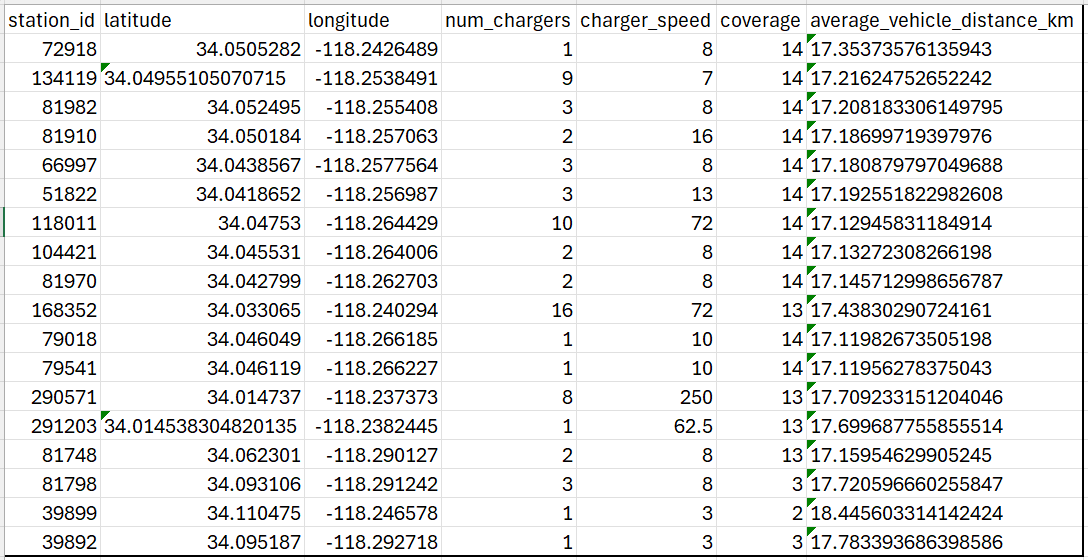
\includegraphics[width=\textwidth]{../Figures/evcs_dataset.PNG}
    \caption{EVCS Dataset}
    \label{fig:EVCS Dataset}
\end{figure}
\newline


To ensure the efficiency of an electric vehicle charging station (EVCS) network, it is essential that stations meet Level 3 charger standards (\(\geq 50\)~kW). In the context of solving a multi-objective optimization problem (MOOP) using NSGA-II, this requirement is addressed by adjusting any charger speeds below 50 kW to 50 kW. This ensures that all selected stations are at least Level 3 chargers, directly supporting the goal of maximizing the charger speed. By applying this rule, we avoid solutions that might result from slower chargers and ensure that the optimization algorithm remains focused on achieving the best possible performance across all objectives.



\subsubsection*{Step 2: Define the Multi-Objective Optimization Problem} 
In this step, the electric vehicle charging station (EVCS) problem was formulated as a multi-objective optimization problem with five conflicting objectives: (1) maximizing geographical coverage to ensure that as many demand points as possible are served by at least one station; (2) maximizing charger speed to reduce waiting times for electric vehicle (EV) users; (3) minimizing the number of installed charging stations to lower infrastructure costs; (4) minimizing the total number of chargers to manage costs and operational complexity; and (5) minimizing the average distance between EVs and their nearest EVCS to enhance accessibility and convenience.


To implement this formulation, we used the DEAP framework\cite{Evolutionary algorithms made easy}. The problem was modeled using a custom fitness class where the objectives were assigned specific weights: positive weights (1.0) for maximizing coverage, positive weights (1.0) for maximizing charger speed, negative weights (-1.0) for minimizing the number of stations and negative weights (-1.0) for minimizing the number of chargers, and (-1.0) for minimizing the average distance between EV, and the nearest EVCS. This formulation allows the algorithm to simultaneously balance service quality and cost efficiency. Each individual in the population represents a unique combination of selected charging stations, and the fitness evaluation returns values to each of the four objectives. 


\subsubsection*{Step 2: Define, and initialize DEAP Components}

In this step, the DEAP framework is utilized to define the requirement components for the evolutionary algorithm, such as the fitness function, individual structure, and algorithm settings. These settings include population size, selection strategy, and the methods for crossover and mutation. To initialize these components, we first create a toolbox using DEAP's base.Toolbox. The toolbox is then populated with several registered functions that define the operations for the evolutionary process.

In additon, the individual function is registered to generate an individual from a specified structure using the tools.initIterate method. The population function initializes the population by creating multiple individuals through tools.initRepeat. The mate function, which controls the crossover operation, is defined with the cxTwoPointCheck method. Similarly, the mutation operation is defined using mutShuffleIndexesCheck with a mutation probability. For selection, the selNSGA2 method is registered, which ensures that the selection process follows the NSGA-II strategy for multi-objective optimization. 

Howerver, the evaluate function is linked to the toolbox to evaluate individuals based on their fitness values.

By registering these functions, the necessary components of the evolutionary process are prepared, allowing the algorithm to run efficiently.

\subsubsection*{Step 3: Define Objective Functions}

In this step, we formally define the objective functions that guide the optimization process. The electric vehicle charging station (EVCS) planning problem is formulated as a multi-objective optimization problem comprising five conflicting objectives, as outlined in Section~\ref{subsec:objective-functions}. These objectives are: (1) maximizing geographical coverage, ensuring that electric vehicle (EV) demand points are within the service radius of at least one station; (2) maximizing charger speed to reduce wait times and improve service efficiency; (3) minimizing the number of installed charging stations to manage infrastructure costs; (4) minimizing the total number of chargers to reduce both deployment and operational expenses; and (5) minimizing the average distance between EVs and their nearest station to enhance accessibility. Each objective is mathematically formulated and encoded in the optimization model. The DEAP library is used to implement the problem, where objectives are assigned directional weights to appropriately guide the NSGA-II algorithm during the optimization process.
\newline
These algorithmic objectives help strike a balance between coverage and efficiency by considering the distance between stations, the distance between users and EVCS, charging speed, as well as the number of stations and chargers. This approach leads to optimized solutions that meet the operational needs of the charging network while also reducing overall infrastructure costs, ensuring cost-effective and efficient deployment.
\newline
\subsubsection*{Step 4: Define the evaluation function that combines all objectives}
The evaluation function plays a critical role in guiding the evolutionary algorithm by assessing the quality of each solution based on multiple objectives\cite{Multi-Objective Optimization using Evolutionary Algorithms}. In this step, we define a function that combines all four previously established objectives to evaluate each individual in the stations dataset in the population. The individual represents a selection of electric vehicle charging stations.

The evaluation function calls five separate methods, as discussed in Subsection 3 in this chapter:

\begin{enumerate}
    \item \textbf{Coverage}: Calculated using the \texttt{calculate\_coverage} method, it sums the distances between all unique pairs of selected stations to check station placement across the area.
    
    \item \textbf{Charger Speed}: Determined using the \texttt{calculate\_charger\_speed} method, this objective selects the highest available charging speed among the chosen stations to enhance charging efficiency.

    
    \item \textbf{Number of Stations}: Computed with \texttt{calculate\_num\_stations}, this counts the selected stations, encouraging minimal infrastructure to reduce overall costs.
    
    \item \textbf{Number of Chargers}: Using \texttt{calculate\_num\_chargers}, this sums all chargers at selected stations to further minimize overall costs.

    \item \textbf{Minimize Average Distance}: Computed with \texttt{calculate\_avg\_ev\_distance}, this objective minimizes the average distance between electric vehicles (EVs) and their nearest charging station. A lower average distance improves accessibility, ensuring that stations are efficiently placed to reduce travel time for EV users.
    
\end{enumerate}

The function returns a tuple containing these five values. These outputs are then used by the NSGA-II algorithm within DEAP to rank and evolve the population toward optimal solutions that balance all objectives effectively\cite{Multi-Objective Optimization using Evolutionary Algorithms}.


\subsubsection*{Step 5: Create a random individual with fewer stations selected}
The create\_individual function is responsible for generating a random initial solution, or “individual,” for the evolutionary algorithm. Each individual represents a subset of electric vehicle charging stations selected from the dataset.

In this function, a random number of stations is selected, in range from one to half of the total available stations. This approach creates diverse solutions some with fewer stations and others with more. This allowing the algorithm to explore a wide range of possible solution during optimization.


To create the individual, the function uses Python’s random.sample() to select a unique set of station indices without replacement. This avoids selecting the same station more than once and keeps each solution valid. The result is a list of station numbers that can be checked using the objective functions.


Generating a diverse population of individuals is essential in evolutionary algorithms such as NSGA-II\cite{Introduction to evolutionary computing. Springer}. This approach helps the algorithm explore more options, and avoid getting stuck in poor solutions too early. The function keeps the population diverse by randomly changing how many stations are picked and which ones are included. These randomly created station groups form the starting point for the algorithm to begin finding the best charging station solution.


\subsubsection*{Step 6: Apply Genetic Operators and Evolve Population}

In this step, the algorithm improves the population by applying genetic operators: selection, crossover, and mutation. NSGA-II is used for selection, favoring individuals that balance multiple objectives while maintaining diversity\cite{A Fast and Elitist Multi-objective Genetic Algorithm: NSGA-II}. 


The crossover operation is performed during the evolutionary process using the crossover function registered in the toolbox. Typically, a two-point crossover method (cxTwoPoint) is used, which exchanges segments between two parent solutions to produce offspring \cite{Introduction to evolutionary computing. Springer}. Before crossover, checks ensure the parents have sufficient length to apply this operation correctly, maintaining solution validity and diversity in the population \cite{Introduction to evolutionary computing. Springer}. 

In addition, the mutation is handled by mutation function registered in the toolbox,which introduces small random changes to individuals by occasionally removing a station. This reduces the number of stations, promoting simpler, more efficient solutions. It also helps prevent duplicate values and ensures that each individual remains a valid configuration\cite{Introduction to evolutionary computing. Springer}. These operations are repeated over generations, allowing the population to explore new combinations, avoid premature convergence, and evolve toward optimal\cite{Introduction to evolutionary computing. Springer} electric vehicle charging station solution.

\section{Performance Metrics}

To evaluate the effectiveness of the multi-objective optimization approach for electric vehicle charging station (EVCS) placement, several performance metrics were used. These metrics reflect both the algorithm’s ability to generate high-quality solutions and the trade-offs between conflicting objectives:

\begin{itemize}
    \item \textbf{1. Pareto Front Coverage}: Measures how well the obtained solutions approximate the ideal Pareto front. A higher coverage indicates a broader and more complete set of trade-off solutions.

    \item \textbf{2. Convergence and Diversity}: Evaluates how close the solutions are to the optimal front (convergence) and how evenly they are distributed across it (diversity), ensuring both quality and variety in trade-off options.

    \item \textbf{3. Area Coverage}: Assesses the percentage of the region effectively served by charging stations. This metric directly relates to the objective of maximizing coverage but may trade off against the number of stations and chargers.

    \item \textbf{4. Average Distance}: Represents the mean distance between EVs and their nearest charging station. Minimizing this improves accessibility but may require more stations or higher-speed chargers, affecting cost.

    \item \textbf{5. Charger Cost}: Estimates the total cost of installing and operating the charging infrastructure, influenced by both the number and type (speed) of chargers. This metric often conflicts with goals such as maximizing coverage and minimizing average distance.
\end{itemize}



